\documentclass[12pt]{article}

\usepackage{amsmath}
\usepackage{amssymb}
\usepackage{amsthm}
\usepackage{graphicx}
\usepackage{float}

\title{An Introduction To\\Conformal Geometric Algebra}
\author{Spencer T. Parkin}

\newcommand{\G}{\mathbb{G}}
\newcommand{\V}{\mathbb{V}}
\newcommand{\R}{\mathbb{R}}
\newcommand{\B}{\mathbb{B}}
\newcommand{\nvao}{o}
\newcommand{\nvai}{\infty}

\newtheorem{theorem}{Theorem}[section]
\newtheorem{definition}{Definition}[section]
\newtheorem{corollary}{Corollary}[section]
\newtheorem{identity}{Identity}[section]
\newtheorem{lemma}{Lemma}[section]
\newtheorem{result}{Result}[section]

\begin{document}
\maketitle

Conformal geometric algebra is a model of
geometry implemented in the language of geometric algebra.
This document is my attempt to rigorously build the
conformal model from the ground up.
It is only assumed that the reader is familiar with geometric algebra.
I used the books $\cite{dorst07}$ and $\cite{hestenes87}$
to learn geometric algebra and the conformal model.
I recommend them for further study.

\section{Representing Geometry}

We begin by defining how geometries are represented in the model.
Letting $\R^n$ denote $n$-dimensional Euclidean space, we will
represent geometries as subsets of this space.  Having done so,
we may perform unions, intersections and other operations of geometries, but we
have no easy means of performing any geometric analysis.  Measurements, normals,
tangents, centers, shape and other things that may characterize a geometry are not
so easily gleaned or inferred from a set of points.  This is where
geometric algebra comes in.

Letting $\G$ denote the geometric algebra to be used by our model
of geometry, we begin by letting $p:\R^n\to\G$ be a vector-valued
function of a Euclidean point, the definition of which we leave
open for the moment.  We then use this function in the following definition.
\begin{definition}\label{def_direct_rep}
For any blade $B\in\G$, we say that $B$ directly
represents a geometry as the set of points
$G(B)=\{x\in\R^n|p(x)\in B\}$.
\end{definition}
Recall that for any vector $v\in\G$, we say that $v\in B$ if and only if $v\wedge B=0$.
Clearly this means that $v$ is in the vector space spanned by any vector factorization
of $B$.  Letting $B^*$ denote a dual of $B$, it is not hard to show that
$v\in B^*$ if and only if $v\cdot B=0$.
\begin{definition}\label{def_dual_rep}
For any blade $B\in\G$, we say that $B$ dually
represents a geometry as the set of points
$G^*(B)=\{x\in\R^n|p(x)\in B^*\}$.
\end{definition}
Notice that by any one of these two definitions, if $B$ represents
a given geometry, then so does $B^*$ by the other definition.
That is, $G^*(B)=G(B^*)$.
Furthermore, any non-zero scalar multiple of $B$ is also representative
of the same geometry.  That is, for all non-zero $\lambda\in\R$,
we have $G(B)=G(\lambda B)$.

\section{Operations of Geometry}

Noticing that the set of all blades in $\G$ is closed under the
outer product operation of geometric algebra,
a natural question arrises as to what geometries are represented
by the results of this operation in terms of
the geometries directly or dually represented by its operands.  To begin to answer this,
we start with a theorem.
\begin{theorem}\label{thm_intersect}
For any vector $v\in\G$ and any two blades $A,B\in\G$,
if $A\wedge B\neq 0$, then $v\cdot A=0$ and $v\cdot B=0$ if and only if $v\cdot A\wedge B=0$.
\end{theorem}
\begin{proof}
If $A\wedge B\neq 0$, then $A\wedge B$ represents the union of the vector sub-spaces
represented by $A$ and $B$.  Stating the next part of the theorem another way, we can
say that $v\wedge AI=0$ and $v\wedge BI=0$ if and only if $v\wedge (A\wedge B)I=0$,
which is also to say that $v\not\in A$ and $v\not\in B$ if and only if $v\not\in A\wedge B$.
\end{proof}
If $A\wedge B=0$, then the calculation of the union of the vector sub-spaces represented by
$A$ and $B$ is a bit more involved, but is a more general formula for what we call the join
of $A$ and $B$.  The meet operation gives us the blade representative of the interesection
of the represented vector sub-spaces. The more general meet and join
operations may have their uses in the conformal model, but here we will stick to the
simpler case of the join operation for now.

We can apply theorem $\eqref{thm_intersect}$ to get the following result.
\begin{result}\label{rslt_intersect}
For any two blades $A,B\in\G$ such that $A\wedge B\neq 0$, we have
\begin{equation*}
G^*(A)\cap G^*(B) = G^*(A\wedge B).
\end{equation*}
\end{result}
Interestingly, we see here that the outer product gives the
dual representation of the intersection between the two geometries
dually represented by the blades taken in that product.
\begin{theorem}\label{thm_union_and_more}
For any vector $v\in\G$ and any two blades $A,B\in\G$,
if $v\wedge A=0$ or $v\wedge B=0$, then $v\wedge A\wedge B=0$.
\end{theorem}
\begin{proof}
If $A\wedge B=0$, then we're done.  If $A\wedge B\neq 0$ and $v\in A$ or $v\in B$,
then $v\in A\wedge B$, which is to say that $v$ is in the union of the vector sub-spaces
represented by $A$ and $B$.
\end{proof}
To see why the converse of theorem $\eqref{thm_union_and_more}$ does not generally hold,
realize that if $v\in A\wedge B$, then $v$ is contained within a vector sub-space of
$A\wedge B$ that might non-trivially overlap both $A$ and $B$, showing that $v\not\in A$ and
$v\not\in B$.

Applying theorem $\eqref{thm_union_and_more}$, we get the following result.
\begin{result}\label{rslt_union_and_more}
For any two blades $A,B\in\G$, we have
\begin{equation*}
G(A)\cup G(B)\subseteq G(A\wedge B).
\end{equation*}
\end{result}
Here we see that the outer product gives the direct representation
of a geometry that is at least the union of the geometries directly
represented by the blades taken in that product.  Unlike the intersection
result given earlier, however, here we cannot come to any certain conclusion
about what is being represented, even if we know exactly what
geometries are being represented by the operands of the operation.
To resolve this, we'll find a relationship between the geometries
generated through the use of the intersection operation and the geometries
generated through the use of the union-like operation.

\section{Generating Geometry}

Having not yet defined the function $p(x)$ or the signature of our
geometric algebra $\G$, what we have covered so far applies to
any number of possible models of geometry based upon geometric algebra.
Therefore, to start getting specific about geometry in our model,
we will now give an explicit formula for $p(x)$ and define $\G$.
As part of this, we will embed $\R^n$ in $\G$.  Notice, however, that
this is not a requirement of the generalized model, but it is how
the conformal model works.
We do this by replacing $\R^n$
with an $n$-dimensional Euclidean vector space $\V^n$, (interpreting
Euclidean vectors as Euclidean points in the usual manner), and
make the geometric algebra generated by this vector space
a sub-algebra of $\G$.  Specifically, if $\{e_k\}_{k=1}^n$ is
any set of $n$ basis vectors for $\V^n$, then a set of
basis vectors for a vector space we'll denote by $\V$ generating $\G$
is given by $\{\nvao,\nvai\}\cup\{e_k\}_{k=1}^n$, where $\nvao$ and $\nvai$ are
refered to as the null vectors
at the origin and infinity, respectively.
\begin{definition}
For any vector $v\in\V$, if $v\cdot v=0$, we call $v$ a null vector.
\end{definition}
The null vectors $\nvao$ and $\nvai$ obey the relationship
$\nvai\cdot\nvao=-1$.  Furthermore, for
all vectors $v\in\V^n$, we define $v\cdot\nvao=0$ and $v\cdot\nvai=0$.

Having precisely defined our geometric algebra $\G$, we define
$p:\V^n\to\G$ as follows.
\begin{equation*}
p(x) = \nvao + x + \frac{1}{2}x^2\nvai
\end{equation*}
It is now not hard to show that for any $x\in\V^n$, the vector $p(x)$
both directly and dually represents the Euclidean point $x$.  We leave
this as an exercise
for the reader, as well as showing that for any scalar $r>0$, that
$p(x)-\frac{1}{2}r^2\nvai$ dually represents an $n$-dimensional hyper-sphere
at $x$ with radius $r$.  The reader should also convince themselves that a
vector of the form $v+(x\cdot v)\nvai$ dually represents an $(n-1)$-dimensional
hyper-plane containing the
point $x$ and being orthogonal to the unit-normal $v\in\V^n$.

Now having blades that represent the spheres and planes in the highest possible
dimensions of interest in $n$-dimensional Euclidean space, let us now apply
the intersection result $\eqref{rslt_intersect}$ to generate as many round
and flat geometries as we can.  Doing so, we see that we can generate
hyper-spheres and hyper-planes of dimensions $0$ through $n-1$ as
outer products of vectors.  For $n=3$, the following table summerizes
the geometries we find and the grades of the blades dually representing them.
\begin{equation*}
\begin{array}{ccccccc}
\mbox{Grade} & \vline & \mbox{Degenerate Dual Round} & \vline & \mbox{Dual Round} & \vline & \mbox{Dual Flat} \\
\hline
1 & \vline & \mbox{Point} & \vline & \mbox{Sphere} & \vline & \mbox{Plane} \\
2 & \vline & \mbox{Tangent-Point} & \vline & \mbox{Circle} & \vline & \mbox{Line} \\
3 & \vline & \mbox{Tangent-Point} & \vline & \mbox{Point-Pair} & \vline & \mbox{Flat-Point}
\end{array}
\end{equation*}
There is nothing more or less that characterizes a flat-point in comparison
to a regular point, which may be thought of as a round-point, also being
a degenerate sphere (a sphere of radius zero).  Flat-points are called flat,
because they're the first entry in the list of flat geometries in order of
increasing dimension.  (Flat-point, line, plane, hyper-plane, etc.)

At first glance, the point-pair may seem out-of-place, but it is simply
the 1-dimensional analog of a sphere or circle.  It has a center and
a radius, but only two points.

The dual tangent point of grade 2 is a degenerate
circle, and the dual tangent point of grade 3 is a degenerate point-pair.
These occur when we intersect a plane in one point on a round,
which is why they're called tangent points.

Using the intersection result $\eqref{rslt_intersect}$ with $n$-dimensional spheres
and $(n-1)$-dimensional planes, we come to the following result relating the grade of a blade
with the geometry dually represented by that blade.
\begin{result}\label{rslt_intersect_grades}
If $B\in\G$ is a blade dually representative of an $m$-dimensional
hyper-sphere, then the grade of $B$ is $n-m+1$.  If $B\in\G$ is a blade
dually representative of an $m$-dimensional hyper-plane, then the
grade of $B$ is $n-m$.
\end{result}

A close look at the vector forms of $n$-dimensional spheres and $(n-1)$-dimensional
planes will reveal that we have exhausted all the types of geometries that we can
represent using a vector.  (Imaginary spheres will be treated in a later section.)
Let us now turn our attention to the method of generating
geometries using the union-like result $\eqref{rslt_union_and_more}$.  Interestingly, what we'll
find is that we can generate the above geometries using this method.
We start with a definition.
\begin{definition}\label{def_co_hyper_planar}
For all $m\geq 0$, we say that the $m+2$ points $\{x_k\}_{k=1}^{m+2}\subset\V^n$
are co-$m$-hyper-planar under the following circumstances.
\begin{equation*}
\begin{array}{l}
\mbox{For $m=0$, the points are identical.} \\
\mbox{For $m=1$, the points are co-linear.} \\
\mbox{For $m=2$, the points are co-planar.} \\
\mbox{For $m=3$, the points are co-hyper-planar.} \\
\mbox{etc.}
\end{array}
\end{equation*}
Here, $m$ corresponds to the dimension of the flat upon which all $m+2$
points lie.
\end{definition}
We then need the following theorem.
\begin{theorem}\label{thm_fit_round}
For any set of $m\geq 2$ points $\{x_k\}_{k=1}^m\subset\V^n$, if these
$m$ points are non-co-$(m-2)$-hyper-planar, then the set of $m$ vectors in $\{p(x_k)\}_{k=1}^m$
are linearly independent.
\end{theorem}
\begin{proof}
Put proof here.
\end{proof}
Using this theorem, it is now not hard to show that blades directly representative
of non-degenerate rounds of the conformal model have factorizations in
terms of vectors representative of points.  To see this, let $B\in\G$ be
a blade directly representative of an $m$-dimensional round, where $m>0$.  Now convince yourself
that $m+1$ points can be found on the surface of this round that are also
non-co-$(m-1)$-hyper-planar.  The vectors representative of these
points are therefore linearly independent (by theorem $\eqref{thm_fit_round}$) and
in the vector space represented by $B$ (by definition $\eqref{def_direct_rep}$).
All that remains then, to show that $B$ is a scalar multiple of the outer product
of these vectors, is that the grade of $B$ is $m+1$.  Knowing that the round in question
here is $m$-dimensional, we see that $B^*$ is of grade $n-m+1$ by result $\eqref{rslt_intersect_grades}$.
The grade of $B$ is therefore $n+2-(n-m+1)=m+1$.

For the case $m=0$, notice that the 0-dimensional round is the degenerate $n$-dimensional round
or point.  A factorization is trivially known as a vector representative of the point.

We now see that we can build up the rounds of the conformal model using
the outer product of vectors representative of points.  In fact, we now see
that it may be more accurate to think of this as a fitting operation instead of
a union-like operation.  Observe that the conformal model not only easily and
naturally solves the problem of fitting an $m$-dimensional hyper-sphere
to a set of $m+1$ points, but it also allows us to think of the blade directly
representative of that sphere in terms of any appropriate factorization
of vectors representative of points on that sphere.  We
can choose any $m+1$ points on the sphere to be in the outer product, provided they uniquely
determine the sphere.  We'll see examples of how this idea is
useful when we later solve certain problems using the conformal model.

Of course, not all sets of $m+1$ points determine
an $m$-dimensional hyper-sphere.  In the cases where these points don't determine a sphere, what do
we get?  To answer this question, we need to start with another definition.
%Well, we already know that if the $m+1$ points are co-$(m-1)$-hyper-spherical,
%then the outer product of the vectors directly representative of those points must be zero.
\begin{definition}\label{def_co_hyper_spherical}
For all $m\geq 0$, we say that the $m+2$ points $\{x_k\}_{k=1}^{m+2}\subset\V^n$
are co-$m$-hyper-spherical under the following circumstances.
\begin{equation*}
\begin{array}{l}
\mbox{For $m=0$, the points are identical.} \\
\mbox{For $m=1$, the points are co-point-pair.} \\
\mbox{For $m=2$, the points are co-circular.} \\
\mbox{For $m=3$, the points are co-spherical.} \\
\mbox{For $m=4$, the points are co-hyper-spherical.} \\
\mbox{etc.}
\end{array}
\end{equation*}
Here, $m$ corresponds to the dimension of the non-degenerate round upon
which all $m+2$ points lie.
\end{definition}

For the case $m=1$, if 3 points are non-co-point-pair, (which is to say that
they are non-co-$m$-hyper-spherical), then no two of those points are identical.
That is, they are pair-wise distinct.

With definition $\eqref{def_co_hyper_spherical}$ in place, consider $B\in\G$ as a blade directly representative
of an $m$-dimensional flat, where $m>0$.  Now convince yourself that $m+2$ points can
be found on the surface of this flat that are non-co-$(m-1)$-hyper-planar
and non-co-$m$-hyper-spherical.  By the first of these two conditions,
we know that there exists a subset of size $m+1$ of the $m+2$ points that
determines an $m$-dimensional hyper-sphere in the $m$-dimensional hyper-plane.
The second of these two conditions insures that the outer product
of the blade directly representative of this $m$-dimensional round
with the vector representative of the remaining point of the $m+2$
points is non-zero.  It follows that the vectors representative
of the $m+2$ points form a linearly independent set.  Then since
these points are on the hyper-plane, all that remains to be shown
to see that the outer product of the vectors representative of these
points is a scalar multiple of $B$ is to show that the grade of $B$ is $m+2$.
Knowing that the flat in question here is $m$-dimensional, we see that $B^*$
is of grade $n-m$ by result $\eqref{rslt_intersect_grades}$.
The grade of $B$ is therefore $n+2-(n-m)=m+2$.

For the case $m=0$, the case of flat-points, this argument doesn't work since clearly
one cannot find two unique points on a point.  Fortunately, a bit of work will show
that a flat point is directly represented by a 2-blade of the form $B=\lambda(i+xi\wedge\nvai)I$,
which simplifies to $B=\lambda(1-x\wedge\nvai)\nvao\wedge\nvai$.  (Here, $i$ is
the unit psuedo-scalar of the geometric algebra genearted by $V^n$ and $I$ is
the unit psuedo-scalar of $\G$.)  It follows that
$\nvai\in B$.  Then since we can clearly find a vector representative of a point
that is on the flat-point, we see that $B$ factors as a scalar multiple of the outer
product of this vector and $\nvai$.  (Note that no vector representative of a point
is a scalar multiple of $\nvai$.)

Interestingly, what we've learned so far is that all geometries,
with the exception of flat points, can be written as outer products
of vectors representative of points.  Our next result, however, will
show that we can represent direct flat geometries in what might be
considered a more convenient way.
\begin{theorem}\label{thm_round_to_flat}
If a blade $B\in\G$ directly represents an $m$-dimensional round,
then $B\wedge\nvai$ directly represents the $m$-dimensional flat
containing this $m$-dimensional round.
\end{theorem}
\begin{proof}
Put proof here.
\end{proof}

\section{Solving for Geometry}

Knowing how geometries of the conformal model factor in terms of vectors
representative of points leads us to one of the reaons why the conformal model
is a powerful analytical tool in geometry.  Specifically, if we're given two blades $A,B\in\G$ that
we know are both directly representative of the same non-single-point geometry, then we can easily show
that $A$ is a scalar multiple of $B$.  Let us state this formally with a theorem.
\begin{theorem}\label{thm_same_geos}
For any two blades $A,B\in\G$, if $G(A)=G(B)$ and these are not singletons,
then there exists a scalar $\lambda\in\R$ such that $A=\lambda B$.
\end{theorem}
\begin{proof}
With the exception of points and flat-points,
if $A$ and $B$ both directly represent the same geometry,
then any factorization of $A$ in terms of vectors representative of points will
also be, up to scale, a factorization of $B$.
\end{proof}
This is a powerful result, because the formulation
of $A$ may have been made one way, while the formulation of $B$, another, and now
we have found a way to relate the two formulations.  For example,
we might formulate $A$ as the intersection between two spheres.  Our result then tells us
that we can interpret $A$ as we would write the geometry represented by $A$ in a
canonical form $B$.  After composing $A$, we can decompose it as we would $B$.

Right away we can use theorem $\eqref{thm_same_geos}$ to come up with an important result.
\begin{theorem}\label{thm_flat_xor_round}
A blade $B\in\G$ directly represents a flat geometry if and only if
$B\wedge\nvai=0$.
\end{theorem}
\begin{proof}
By the previous section and theorem $\eqref{thm_round_to_flat}$, if the blade $B$ directly represents a round,
then $B\wedge\nvai$ represents a flat.  But also by the previous section, we know that the
flat directly represented by $B\wedge\nvai$ can also be directly represented by an outer
product of vectors representative of points on the flat.  But by theorem $\eqref{thm_same_geos}$, these blades
are scalar multiples of one another.  Therefore, in any case, the outer product of $\nvai$
and a factorization of this flat must be zero.

Prove other direction here.
\end{proof}
Notice that this theorem can also be stated as follows.  A blade $B\in\G$
directly represents a round geometry if and only if $B\wedge\nvai\neq 0$.
This is because every geometry is either round or flat.

Another useful feature of the conformal model comes from the way it lets
us think about doing operations at a high level.  We needed only descend to
the lower levels of thinking to develop the model.  Once developed, what we can do now is illustrated
by the following example.  Suppose we're given a dual circle $A$ and
a point $B$, and we want to find the dual sphere $C$ fitting these two geometries.
Well, we can think of $A^*$ as any three points determining the circle.
Combining this in the outer product with $C$, we then see that we
get what may be four points that determine the desired sphere.
Finally, we can come to the conclusion that $C=(A^*\wedge B)^*=A\cdot B$,
which is a nice result!  Our answer is simply the inner product of the two blades
representing the geometries in question.  Furthermore, the blade $C$ gives
us useful information in all situations.  If $C=0$, then $B$ was on $A$.
If $C\wedge\nvai=0$, then the sphere is really a plane and we may
think of it as centered at infinity with radius infinity.  In the remaining case, $C$ is
a finite sphere.

\section{Transforming Geometry}

Here we study the transformations of conformal geometries
by versors.  Let us therefore give a formal definition of such
elements.
\begin{definition}
Given any set of $m$ invertible vectors $\{v_k\}_{k=1}^m\subset\G(\V)$,
the element
\begin{equation*}
V = \prod_{k=1}^m v_k
\end{equation*}
is called a versor.
If $m$ is odd, we call $V$ an odd versor; if even, an even versor.
I will refer to $m$ as the grade of the versor $V$.
\end{definition}
It follows that versors are invertible by definition.  Clearly $V^{-1}=\tilde{V}/|V|$,
where $|V|=\prod_{k=1}^m |v_k|$.  It is also easy to see that versors
form their own group under the geometric product.  With versors as representative
of transformations, this property allows us to easily concatinate transformations.
As we'll come to find out, we can represent any conformal transformation with
a versor.  This is where the conformal model gets its name.

We will now proceed to lay some ground work
for a very import result that will help us decipher the action of versors on elements
representative of conformal geometries.

\begin{lemma}\label{lma_vector_invariance}
For any vector $a\in\V$, we have $VaV^{-1}\in\V$.
\end{lemma}
\begin{proof}
Notice that we need only show that for any vector $v\in\V$, we have $vav^{-1}=vav/|v|\in\V$.
By the equation
\begin{equation*}
vav = v(a\cdot v + a\wedge v) = (a\cdot v)v + v\cdot(a\wedge v)  = 2(a\cdot v)v - |v|^2a,
\end{equation*}
clearly this is the case.
\end{proof}
\begin{lemma}\label{lma_inner_prod_preserve}
Given any two vectors $a,b\in\V$, we have $VaV^{-1}\cdot VbV^{-1}=a\cdot b$.
\end{lemma}
\begin{proof}
It suffices to show that $\langle V(a\wedge b)V^{-1}\rangle_0=0$, since
\begin{equation*}
VaV^{-1}\cdot VbV^{-1} = \langle VabV^{-1}\rangle_0 = a\cdot b + \langle V(a\wedge b)V^{-1}\rangle_0.
\end{equation*}
A proof by induction is given.  Consider first $\langle v(a\wedge b)v^{-1}\rangle_0$, where $v\in\V$.
By direct evaluation, we get
\begin{equation*}
\langle v(a\wedge b)v^{-1}\rangle_0 = \frac{1}{|v|}
\left|\begin{array}{cc} n\cdot a & n\cdot a\\ n\cdot b & n\cdot b\end{array}\right| = 0.
\end{equation*}
Suppose now that for a fixed integer $k$, the versor $V$
of grade $k$ satisfies the lemma.  We must show that $\langle vV(a\wedge b)V^{-1}v^{-1}\rangle_0$ is zero.
To that end, it is not hard to see that
\begin{equation*}
\langle vV(a\wedge b)V^{-1}v^{-1}\rangle_0 =
\langle v\langle V(a\wedge b)V^{-1}\rangle_0 v^{-1}\rangle_0 +
\langle v\langle V(a\wedge b)V^{-1}\rangle_2 v^{-1}\rangle_0.
\end{equation*}
Clearly $\langle v\langle V(a\wedge b)V^{-1}\rangle_0 v^{-1}\rangle_0$ is zero by our inductive hypothesis.
That $\langle v\langle V(a\wedge b)V^{-1}\rangle_2 v^{-1}\rangle_0$ is zero follows directly from
the work we did to show that $\langle v(a\wedge b)v^{-1}\rangle_0$ is zero.
\end{proof}
We're now ready to prove a theorem that we'll use to prove something very interesting
about versor transformations in the conformal model.
\begin{theorem}\label{thm_outer_prod_preserve}
Given any $m$-blade $B=\bigwedge_{k=1}^m b_k$, we have
\begin{equation*}
VBV^{-1} = \bigwedge_{k=1}^m Vb_iV^{-1}.
\end{equation*}
\end{theorem}
\begin{proof}
Our proof of this theorem will rely upon the following.  If we find that $B=f(b_1,\dots,b_m)$,
where $f$ is any expression in the vector variables $b_1$ through $b_m$, then
clearly
\begin{equation*}
f(Vb_1V^{-1},\dots,Vb_mV^{-1})=\bigwedge_{k=1}^m Vb_iV^{-1}
\end{equation*}
by lemma $\eqref{lma_vector_invariance}$.
All that would remain, then, is to show that
\begin{equation*}
VBV^{-1}=f(Vb_1V^{-1},\dots,Vb_mV^{-1}),
\end{equation*}
and the theorem goes through.

We procede now by strong induction.  Clearly the theorem holds for the case $m=1$.
The case $m=2$ is not much harder to prove.
Suppose now that for a fixed integer $m>2$, that the theorem holds for each case less
than $m$.  A partial expansion of $VBV^{-1}$ gives us
\begin{equation*}
VBV^{-1} = V(b_1\wedge\dots\wedge b_{k-1})b_kV^{-1} - (-1)^{k-1}V(a_k\cdot a_1\wedge\dots\wedge a_{k-1})V^{-1}.
\end{equation*}
We will consider each part of the right-hand side seperately.  For the first part, we have
\begin{align*}
V(b_1\wedge\dots\wedge b_{k-1})b_kV^{-1} &=
V(b_1\wedge\dots\wedge b_{i-1})V^{-1}Vb_kV^{-1} \\
&= \left(\bigwedge_{i=1}^{k-1}Vb_iV^{-1}\right)Vb_kV^{-1},
\end{align*}
by our inductive hypothesis.  For the second part, we have
\begin{align*}
 & (-1)^k V(a_k\cdot a_1\wedge\dots\wedge a_{k-1})V^{-1} \\
 =& -(-1)^k V\left(\sum_{i=1}^{k-1}(-1)^i (a_k\cdot a_i)\bigwedge_{j=1,j\neq i}^{k-1} a_j\right)V^{-1} \\
 =& -(-1)^k\sum_{i=1}^{k-1}(-1)^i (a_k\cdot a_i)V\left(\bigwedge_{j=1,j\neq i}^{k-1} a_j \right)V^{-1} \\
 =& -(-1)^k\sum_{i=1}^{k-1}(-1)^i(Va_kV^{-1}\cdot Va_kV^{-1})\bigwedge_{j=1,j\neq i}^{k-1} Va_jV^{-1},
\end{align*}
by lemma $\eqref{lma_inner_prod_preserve}$ and our inductive hypothesis.
Having now sandwitched all vectors between $V$ and $V^{-1}$, our proof by
induction is complete.
\end{proof}
What theorem $\eqref{thm_outer_prod_preserve}$ tells us is that the function
$f(B)=VBV^{-1}$ is an outermorphism.  Applying this theorem, we get the following
important result.
\begin{result}\label{rslt_versor_action_on_geos}
Given a versor $V$, if we understand the transformation $Vp(x)V^{-1}$ for
any point $x\in\V^n$, then we understand the transformation $VBV^{-1}$,
where $B$ is any blade directly or dually representative of any geometry, with
the only exception being that of flat points.
\end{result}
\begin{proof}
In the previous section we showed that, with the exception of flat points,
all geometries directly represented by a blade $B$ may be written
as the outer product of vectors representative of points.  For all of
these geometries, our result goes through directly by theorem $\eqref{thm_outer_prod_preserve}$.

To show now that the theorem goes through for blades dually representative of geometries, (with again,
the exception of flat-points),
we need only show the commutativity of grade $k$ versors with the unit-psuedo scalar $I$ of $\G$.
For any vector $v\in\V$, it is not hard to show that $vI=(-1)^nIv$.  It follows that $VI=(-1)^{nk}IV$.
We then see that
\begin{equation*}
VBV^{-1} = -VBV^{-1}I^2 = -(-1)^{nk}VBIV^{-1}I,
\end{equation*}
which relates what we already know about the action of versors on blades directly
representative of geometries with those dually representative of such geometries.
\end{proof}
This is a fantastic result!  We now not only have a way of formulating a desired
transformation, but we also know that such a formulation, once formulated, will
apply to almost all geometries in the conformal model, no matter the representation!
This is similar to what we know about linear transformations.  A linear transformation
is entirely determined by how it transforms a basis of the space.  Therefore, if we
know how a desired transformation transforms a basis of the space, then we have
found the desired linear transformation.  Analogously, if we know how a desired
conformal transformation transforms a point, then we have found the desired
conformal transformation.  On the other hand, if we know how a given versor
transforms a point, then we can predict how it will transform any conformal
geometry, except flat points.

Flat points are an exception to the idea presented in result $\eqref{rslt_versor_action_on_geos}$,
because a given versor may not always leave $\nvai$ invariant up to scale.
We'll see an example of this in section $\eqref{sec_spherical_reflections}$ below.

We procede now to develop the versor transformations of the conformal model.

\subsection{Reflections}

Interestingly, what we find in the conformal model is that a vector
not only represents a piece of geometry, but, as a versor, also represents
a transformation involving that geometry.  Specifically, a plane represents
a reflection about that plane, and a sphere represents a reflection about that
sphere!

Reflections turn out to be a very fundamental type of transformation, because
so many other types of transformations, such as rotations and translations, can be described
in terms of reflections about well chosen geometries.  For example, two
successive reflections about two well chosen planes gives us either a rotation
or a translation.  (Interestingly, this shows that the rotation and translation
transformations are perhaps not as disimilar as we might have first thought them to be!)

Another type of reflection is performed about a sphere.  That is, a point
interior to a sphere is reflected out of it, while points exterior to the sphere
are reflected into it.  The question then comes up: if two successive
reflections about two well chosen planes gives us the rotation or
translation transformations, what does two successive reflections about
two well chosen spheres give us?  We will get to the bottom of this question later on.

\subsection{Planar Reflections}

Given a plane centered at $c\in\V^n$ with unit-length normal $v\in\V^n$,
here we consider the action of the vector dually representative of this plane
as a versor on a vector representative of a point.  That is, for $\pi=v+(v\cdot c)\nvai$,
what do we get in the evaluation of $\pi p(x)\pi^{-1}$?  Expanding this out, we get
\begin{equation*}
\pi p(x)\pi^{-1} = -p(y),
\end{equation*}
where $y=x-2(v\cdot (x-c))v$.  Drawing a picture
of this will convince you that $y$ is the reflection of $x$ about the plane!

Interestingly, here we have an example of a versor that leaves $\nvai$
invariant but for a factor of $-1$.  It follows that
\begin{equation*}
\pi(p(x)\wedge\nvai)\pi^{-1} = p(y)\wedge\nvai,
\end{equation*}
showing that flat points reflect about planes the same way round points do.

Having covered the case of flat points, we can now apply result $\eqref{rslt_versor_action_on_geos}$
to find that the versor $\pi$ reflects any conformal geometry about the plane represented by
$\pi$ as we would imagine.  Even a sphere partially straddling the plane will reflect as we would predict.

\subsection{Translations}

It is not hard to imagine that we can perform a translation
using a single planar reflection about a well chosen plane.
The problem with this is that we need a different plane for
every situation.  Interestingly, however, what we'll find is that
if we perform two successive reflections about two parallel planes,
the position of those planes becomes arbitrary, while only the relative
distance between those planes determines the amount of translation.
The direction of translation is determined by the attitude of the parallel planes.

Let $v\in\V^n$ be a unit-normal shared by two parllel planes, let
$c\in\V^n$ be the position of the first plane, and $t\in\V^n$
be a vector representative of the desired amount of translation.
We assume that $v\wedge t=0$.
The versor representative of the translation is then given by
\begin{equation*}
(v+(v\cdot(c+\frac{1}{2}t)\nvai)(v+(v\cdot c)\nvai) = 1 - \frac{1}{2}t\nvai.
\end{equation*}
Notice that our result here is independent of the position of the
first plane, but only dependent upon the relative positions of
the two planes.
Of course, also notice that $v$ goes away as $t$ is all that
is needed to characterize the translation transformation.

% Give polar decomposition?

\subsection{Rotations}

Suppose now that the two planes we reflect about are
non-parallel.  In this case we get a rotation.  Let $c\in\V^n$
be a common point among the two planes, and let $v_0,v_1\in\V^n$
be their unit-normals, respectively.  Not being parallel planes,
we have $v_0\wedge v_1\neq 0$.  We can then let $a\in\V^n$
be a unit-length vector representing the axis of rotation, and
let $\theta\in\R$ be the angle of rotation.  Doing so, we see
that $v_0\wedge v_1=-ai\sin\theta/2$.  The versor that
represents a rotation about the point $c$ is then given by
\begin{equation*}
(v_0+(v_0\cdot c)\nvai)(v_1+(v_1\cdot c)\nvai) = \cos\frac{\theta}{2} - (a+a\wedge c\wedge\nvai)i\sin\frac{\theta}{2}.
\end{equation*}
Letting $c=0$, we get the well-known rotor in Euclidean geometric algebras which
has a polar decomposition of $\exp(-ai\theta/2)$.

% Does our form here have a polar decomposition?

\subsection{Spherical Reflections}\label{sec_spherical_reflections}

Let $c\in\V^n$ be the center of a sphere, and $a\in\V^n$ be a point
exterior to the sphere.  Then the point $b\in\V^n$ along the line
from $c$ to $a$ given in the following figure is what we refer to
as the reflection of $a$ in the sphere.
\begin{figure}[H]\label{fig_spherical_reflection}
\centering
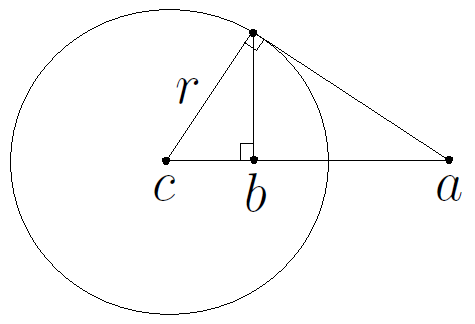
\includegraphics[scale=0.3]{SphericalReflectionFigure}
\caption{The reflection of a point about a sphere.}
\end{figure}
We let $r\in\R$ be the radius of this sphere.  Using what we know about similar
triangles, it is not hard to show that $b = (1-\lambda)c + \lambda a$,
where
\begin{equation*}
\lambda = \left(\frac{r}{|c-a|}\right)^2 = \left(\frac{|c-b|}{r}\right)^2,
\end{equation*}
the square of a common ratio between respective sides of the
similar triangles in the figure above.
Interestingly, letting $s=p(c)-\frac{1}{2}r^2\nvai$ be the sphere in the figure, we find that
\begin{equation*}
sp(a)s^{-1} = -\lambda p(b),
\end{equation*}
showing that vectors dually
representative of spheres perform, as versors in a versor transformation, spherical reflections!

Applying result $\eqref{rslt_versor_action_on_geos}$, we find that $s$, when
acting upon a blade directly representative of a line, gives us the blade directly
representative of the circle that is the reflection of that line in the sphere.  Similarly,
the reflection of a plane in a sphere is a sphere.

Of course, result $\eqref{rslt_versor_action_on_geos}$ doesn't tell us anything about
how $s$ acts on a flat point.  The key, as always, is to see how $s$ acts on $\nvai$.
Investigating this, we find that
\begin{equation*}
s(p(a)\wedge\nvai)s^{-1} = \frac{2}{(c-a)^2}p(b)\wedge p(c),
\end{equation*}
showing that $s$ transforms the flat point at $a$ into the pair of points $b$ and $c$.

\subsection{Uniform Scaling}

It stands to reason that the only types of geometry in the conformal model
that would be affected by a uniform scaling transformation would be the
round geometries.  We might consider flat geometries as already scaled out
to infinity.  In fact, it is not hard to show that all flats remain invariant under
such a transformation.  For any set of points determining a flat of dimension
greater than zero, if they are all scaled away from a common point on the flat, then they
still determine the same flat, provided the scale is reasonable.

% This is two successive reflections about two spheres sharing the same center.

\subsection{Transversion}

%Is this two successive reflections about two well chosen spheres?

% It is two successive reflections about two spheres that touch one another in a single point.

% Logarithm not yet known?

\subsection{Other Transformations}

Yet more types of transformations can be constructed in the conformal model
by combining the above mentioned transformations.  For example, general
rigid body motions can be formulated by combining the rotation and translation
versors.  A question should be answered about the set of all possible types
of transformations and what groups they form under versor concatination, but
this might be beyond the scope of this paper and, admittedly, the capabilities of the author.

In any case, it should be clear that by combining all types of reflection vector versors, (planar and spherical),
that we exhaust all possible transformations by versors that we can come up with in the
conformal model.  We have only begun to discover what types of transformations we
can do with these basic building blocks.  (There are undoubtadly more combinations to
consider.)  But we will leave versor transformations for now, content with what we have
covered thus far as an introduction to the subject.

\section{Catalog of Dual Representations and Versor Transformations}

For reference, this section catalogs canonical dual representations of the geometries in the
conformal model of 3-dimensional space, as well as common transformations represented
by versors.  In each sub-section about dual geometric representations, the blade $B\in\G$ is
assumed to represent the geometry in question, while in sub-sections about
versor transformations, the versor $V\in\G$ represents the transformation in question.
In addition to the composition
of each geometry's dual representation, a sequence of steps
are also provided that show how one can decompose this representation
into the variables that characterize the geometry.  A similar set of composition
and decomposition steps are provided for the versor transformations.

\subsection{Points}

Points (round points) are characterized by a Euclidean point $x\in\V^n$ and
a non-zero scalar (weight) $\lambda\in\R$.
\begin{equation*}
B = \lambda\left(\nvao + x + \frac{1}{2}x^2\nvai\right)
\end{equation*}
We may decompose this as follows.
\begin{align*}
\lambda &= -\nvai\cdot B \\
v &= \nvao\wedge\nvai\cdot\frac{B}{\lambda}\wedge\nvao\wedge\nvai
\end{align*}

\subsection{Spheres}

Spheres are characterized by a Euclidean point (center) $x\in\V^n$, a
non-zero radius $r\in\R$ and a non-zero scalar (weight) $\lambda\in\R$.
\begin{equation*}
B = \lambda\left(\nvao + x + \frac{1}{2}(x^2\pm r^2)\nvai\right)
\end{equation*}
(Say something about imaginary spheres.)
We may decompose this as follows.
\begin{align*}
\lambda &= -\nvai\cdot B \\
x &= \nvao\wedge\nvai\cdot\frac{B}{\lambda}\wedge\nvao\wedge\nvai \\
r^2 &= x^2 + 2\nvao\cdot\frac{B}{\lambda}
\end{align*}
Alternatively, we can find $r^2$ as simply the square of $B/\lambda$.

\subsection{Planes}

Planes are characterized by a Euclidean point (center, if you will) $x\in\V^n$,
a unit-normal $v\in\V^n$ and a non-zero scalar (weight) $\lambda\in\R$.
\begin{equation*}
B = \lambda(v + (x\cdot v)\nvai)
\end{equation*}
If $T=1-\frac{1}{2}x\nvai$, we may also formulate $B$ as $Tv\tilde{T}$.
We may decompose $B$ as follows.
\begin{align*}
v &= \nvao\cdot\frac{B}{\lambda}\wedge\nvai \\
x &= -v\left(\nvao\cdot\frac{B}{\lambda}\right)
\end{align*}
Notice here that any original weight, normal and position used in
the composition of $B$ are not recoverable in the decomposition of $B$.
Here, $x$ will be the point on the plane closest to the origin.

\subsection{Circles}

Circles are characterized by a Euclidean point (center) $x\in\V^n$,
a unit-normal $v\in\V^n$, a non-zero radius $r\in\R$ and a non-zero scalar (weight) $\lambda\in\R$.
\begin{equation*}
B = \lambda(v+(x\cdot v)\nvai)\wedge\left(\nvao+x+\frac{1}{2}(x^2\pm r^2)\nvai\right)
\end{equation*}
(Say something about imaginary circles.)  We may decompose this as follows.
\begin{align*}
v &= \nvao\wedge\nvai\cdot\frac{B}{\lambda}\wedge\nvai \\
x &= v\left(\nvao\wedge\nvai\cdot\frac{B}{\lambda}\wedge\nvao\nvai\right) \\
r^2 &= x^2 - 2v\left((x\cdot v)x-\nvao\wedge\nvai\cdot\nvao\wedge \frac{B}{\lambda}\right)
\end{align*}

\subsection{Lines}

Lines are characterized by a Euclidean point (center, if you will) $x\in\V^n$,
a unit-normal $v\in\V^n$ and a non-zero scalar (weight) $\lambda\in\R$.
\begin{equation*}
B = \lambda\left(vi - \left(x\cdot vi\right)\wedge\nvai\right)
\end{equation*}
We may decompose this as follows.
\begin{align*}
v &= \left(\nvao\cdot\frac{B}{\lambda}\wedge\nvai\right)i \\
x &= -v\left(\nvao\cdot\frac{B}{\lambda}\right)i
\end{align*}

\subsection{Point-Pairs}

Point-pairs are characterized by a Euclidean point (center) $x\in\V^n$,
a unit-normal $v\in\V^n$, a non-zero radius $r\in\R$ and a non-zero scalar (weight) $\lambda\in\R$.
\begin{equation*}
B = \lambda(vi-(x\cdot vi)\wedge\nvai)\wedge\left(\nvao+x+\frac{1}{2}(x^2\pm r^2)\nvai\right)
\end{equation*}
(Say something about imaginary point-pairs.)  We may decompose this as follows.
\begin{align*}
v &= -\left(\nvao\wedge\nvai\cdot\frac{B}{\lambda}\wedge\nvai\right)i \\
x &= -v\left(\nvao\wedge\nvai\cdot\frac{B}{\lambda}\wedge\nvao\nvai\right)i \\
r^2 &= -x^2+2v\left((x\cdot v)v+\left(\nvao\wedge\nvai\cdot\nvao\wedge\frac{B}{\lambda}\right)i\right)
\end{align*}

\subsection{Flat Points}

Flat-points are characterized by a Euclidean point $x\in\V^n$ and a non-zero
scalar (weight) $\lambda\in\R$.
\begin{equation*}
B = \lambda(i+xi\wedge\nvai)
\end{equation*}
We may decompose this as follows.
\begin{align*}
\lambda &= -(B\wedge\nvai)i \\
x &= \left(\nvao\cdot\frac{B}{\lambda}\right)i
\end{align*}

\subsection{Tangent Points}

A tangent-point is characterized by a Euclidean point $x\in\V^n$, a unit-normal $v\in\V^n$
and a non-zero scalar (weight) $\lambda\in\R$.  Dual canonical forms of tangent points for
grades 2 and 3 are given by the dual canonical forms of circles and point-pairs, respectively,
with a radius $r$ of zero.  For example, given any $r>0$, simplyfing the following equation recovers
the dual form of a tangent point for grade 2.
\begin{equation*}
B = \lambda(v+(x\cdot v)\nvai)\wedge\left(\nvao+x-rv+\frac{1}{2}((x-rv)^2-r^2)\nvai\right),
\end{equation*}
The reader will notice that $r$ cancels itself out.  The decomposition steps for tangent
points are the same as those given for circles and point-pairs.  The recovered radius
will be zero in the case of tangent points.

\subsection{Free Blades}

Address free-blades here.

\subsection{Rotate-Translate Transformations}

Such a transformation is characterized by a Euclidean translation vector $t\in\V^n$, a unit-axis $a\in\V^n$,
an angle $\theta\in\R$ and a scalar (weight) $\lambda\in\R$.
\begin{equation*}
V = \lambda\left(1-\frac{1}{2}t\nvai\right)\left(\cos\frac{\theta}{2}-ai\sin\frac{\theta}{2}\right),
\end{equation*}
Notice that $V$ here is not a blade.  It is an even versor.  If the blade $B\in\G$ represents
a geometry, (directyl or dually), the transformation of $B$ by $V$ is given by $VBV^{-1}$,
in the case that we wish to the apply the rotation first, then the translation.
We may decompose this type of transformation as follows.
\begin{align*}
\lambda^2 &= V\tilde{V} \\
R &= -\nvao\cdot\frac{V}{\lambda}\wedge\nvai \\
T &= \frac{V}{\lambda}\tilde{R} \\
\theta &= 2\cos^{-1}\left\langle R\right\rangle_0 \\
a &= \frac{1}{\sin(\theta/2)}\left\langle R\right\rangle_2 i \\
t &= 2\nvao\cdot(1-T)
\end{align*}
(Say something about the polar decomposition of $V$.)

\section{Concluding Remarks}

This introduction has only just begun to scratched the surface of
what kinds of geometry we can do with the conformal model, and
any model like it that uses a homogenous blade representation scheme,
such as the model for projective geometry.  It is reasonable to ask
what other models of geometry there might be that use different
types of geometric algebras.  Instead of going in search of a model
with specific features, we might as well just choose a geometric algebra,
and then ask what types of geometry we can do with that algebra under
various models of geometry.

% Something interesting happens when we interpret something as something it's not.
% For example, interpret a direct point-pair (grade 2) as a dual circle (grade 2).

\bibliographystyle{plain}
\bibliography{CGAIntro}

\end{document}

% How does meet and join perform operations on geometry in the conformal model?